\documentclass[journal]{IEEEtran}

\usepackage{amsmath,amssymb}
\usepackage{booktabs}
\usepackage{multirow}
\usepackage{array}
\usepackage{tabularx}
\usepackage{graphicx}
\usepackage{url}
\usepackage[hidelinks]{hyperref}
\usepackage{tikz}
\usepackage{balance}
\usepackage{xspace}
\usetikzlibrary{arrows.meta,positioning,fit,calc}

\newcommand{\system}{\textsc{ExecWeave}\xspace}
\newcommand{\etal}{et al.}
\newcommand{\na}{\textemdash}
\newcommand{\notnative}{Not native}
\newcommand{\partialcap}{Partial}

\title{ExecWeave: Cross-Layer Execution Provenance for Observable Agentic Software}

\author{Anonymous Author(s)%
\thanks{This manuscript is an initial journal draft. Author information is intentionally omitted from this version.}}

\begin{document}
\maketitle

\begin{abstract}
Large-language-model agents increasingly cross the boundary between conversational software and executable systems: they delegate to sub-agents, invoke tools, launch processes, modify files, and communicate with local or remote services. Existing agent-observability platforms primarily expose application-level traces such as prompts, model calls, tool invocations, and nested spans, whereas operating-system telemetry exposes processes, files, and network activity without necessarily preserving the agent-level intent that caused those effects. This separation creates a \emph{semantic--runtime observability gap}: neither layer alone is sufficient to answer questions such as which agent or tool caused a particular process, file mutation, or network connection, and an unsound fusion can be worse than missing evidence because it can assign an effect to the wrong principal.

We present \system, a local-first observability system that represents provider semantics and independently observed operating-system evidence in a unified, evidence-aware execution graph. Its design keeps raw runtime observations, provider-supplied semantic events, and derived correlations as distinct evidence layers; materializes typed entities and relations without upgrading weak evidence into causal claims; and explicitly leaves ambiguous cross-layer relations unattributed. A conservative correlation procedure links tool declarations to runtime processes only when bounded temporal and executable evidence yield a unique candidate, while an evidence-grade contract distinguishes native causal attribution, sampled process attribution, session correlation, inference, and unknown support. The same canonical graph model drives live and finished views across heterogeneous providers and operating systems.

We position \system against contemporary agent tracing and graph-observability systems, including LangSmith, Langfuse, Phoenix, AgentOps, W\&B Weave, AgentGraph, AgentSeer, AgentTrace, and Graph of Trace, and against distributed tracing and whole-system provenance. We define a controlled evaluation protocol covering reconstruction fidelity, false attribution, cross-provider and cross-OS consistency, failure robustness, overhead, scalability, and analyst utility. Repository-backed preliminary measurements are reported only where a frozen benchmark artifact exists; final competitive results are deliberately left to controlled experiments rather than inferred from feature documentation. The resulting formulation treats observability not as a visualization problem alone, but as an evidence-preserving cross-layer reconstruction problem for agentic software.
\end{abstract}

\begin{IEEEkeywords}
AI agents, observability, execution provenance, runtime tracing, operating-system telemetry, cross-layer attribution, multi-agent systems, execution graphs.
\end{IEEEkeywords}

\section{Introduction}
\IEEEPARstart{A}{gentic} software is changing the unit of execution that developers must understand. A conventional application may call functions and services according to code paths that are known before execution. An agentic application can instead select tools dynamically, delegate work to other agents, issue shell commands, start language runtimes, call local model servers, edit repositories, and contact external endpoints as part of a single user request. The externally visible answer is therefore only the end of a longer execution chain whose intermediate effects may matter for debugging, security, reproducibility, and accountability.

The observability ecosystem has responded rapidly. LangSmith records traces composed of runs and integrates with agent frameworks and OpenTelemetry~\cite{langsmith2026observability,langsmith2026otel}. Langfuse records observations and now renders agent graphs inferred from typed observations and nesting~\cite{langfuse2026agentgraphs,langfuse2026tracing}. Phoenix uses OpenTelemetry and OpenInference to trace model calls, tools, retrieval, and custom application logic~\cite{phoenix2026tracing,phoenix2026otel}. AgentOps organizes agents, language-model calls, actions, and tools into sessions and hierarchical spans~\cite{agentops2026,agentops2026core}, while W\&B Weave records operations and calls, provides trace and graph views, and includes agent-oriented span types~\cite{wandb2026tracing,wandb2026traceview}. Academic systems similarly convert agent execution into analyzable graph structure. AgentGraph transforms traces into knowledge graphs with agents, tasks, tools, data, and human interventions~\cite{wu2026agentgraph}; AgentSeer separates temporal action and component graphs~\cite{wicaksono2026agentseer}; Graph of Trace visualizes fine-grained tool and code-execution events as an incrementally updated directed graph~\cite{gao2026graphtrace}; and AgentTrace proposes structured operational, cognitive, and contextual telemetry for agent systems~\cite{alsayyad2026agenttrace}.

These advances make one claim untenable: an execution graph by itself is no longer novel. More importantly, they expose a different research problem. Agent-level instrumentation describes what an integration point \emph{reported}: an agent emitted a tool call, a framework entered a function, or a model returned a response. Operating-system observation describes what a machine \emph{observed}: a process was created, a file changed, or a socket appeared. The two descriptions are related but not equivalent. A declared shell command does not prove that the corresponding process executed; a file body supplied by a provider hook does not prove an operating-system read; and a process connecting to a network endpoint does not by itself identify which logical agent action requested that connection.

We call this separation the \emph{semantic--runtime observability gap}. It has two consequences. First, semantic-only traces can omit effects below the instrumentation boundary. Second, OS-only telemetry can preserve effects while losing the logical principal or tool invocation that motivated them. Naively joining the two streams by timestamp is unsafe under concurrency, process reuse, wrappers, shell indirection, shared runtimes, or overlapping sub-agent activity. For accountability-oriented observability, a false attribution can be more damaging than an explicit unknown: it can blame Agent A for an effect caused by Agent B.

\system addresses this problem by treating observations as evidence and the graph as a materialized, queryable view of that evidence. Provider/framework semantics, inference-gateway observations, model-runtime observations, and OS-runtime evidence remain distinguishable after graph construction. Derived cross-layer bridges are marked as inferred and non-causal unless stronger telemetry supports a stronger claim. Ambiguous cases produce no bridge rather than a visually convenient but unsupported edge. This design follows a lineage of provenance systems that emphasize faithful derivation histories~\cite{muniswamy2006pass,pohly2012hifi,bates2015lpm,pasquier2017camflow}, while adapting the problem to modern agent runtimes whose relevant identities include agents, sub-agents, tool calls, model requests, provider sessions, processes, files, and network endpoints.

Figure~\ref{fig:gap} illustrates the central distinction. The semantic plane can say that a root agent delegated to a sub-agent and that the sub-agent invoked a tool. The runtime plane can say that a process spawned a child that modified a file and contacted a service. The research problem is not to draw both planes; it is to determine which cross-plane relations are justified, with what evidence, and what should remain unknown.

\begin{figure}[t]
\centering
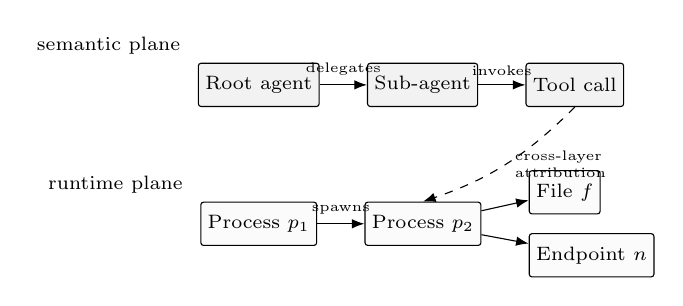
\begin{tikzpicture}[
  node distance=5mm and 6mm,
  box/.style={draw, rounded corners=1pt, align=center, minimum height=5.5mm, inner sep=2.5pt, font=\scriptsize},
  sem/.style={box, fill=gray!10},
  run/.style={box, fill=gray!3},
  arr/.style={-{Latex[length=1.6mm]}, thin},
  bridge/.style={-{Latex[length=1.6mm]}, dashed, thin}
]
\node[sem] (root) {Root agent};
\node[sem, right=of root] (sub) {Sub-agent};
\node[sem, right=of sub] (tool) {Tool call};
\draw[arr] (root) -- node[above,font=\tiny]{delegates} (sub);
\draw[arr] (sub) -- node[above,font=\tiny]{invokes} (tool);

\node[run, below=12mm of root] (p1) {Process $p_1$};
\node[run, right=of p1] (p2) {Process $p_2$};
\node[run, right=of p2, yshift=4mm] (file) {File $f$};
\node[run, right=of p2, yshift=-4mm] (net) {Endpoint $n$};
\draw[arr] (p1) -- node[above,font=\tiny]{spawns} (p2);
\draw[arr] (p2) -- (file);
\draw[arr] (p2) -- (net);
\draw[bridge] (tool.south) to[bend left=13] node[right,font=\tiny,align=left]{cross-layer\\attribution} (p2.north);
\node[font=\scriptsize, anchor=east] at ($(root.west)+(-1mm,5mm)$) {semantic plane};
\node[font=\scriptsize, anchor=east] at ($(p1.west)+(-1mm,5mm)$) {runtime plane};
\end{tikzpicture}
\caption{The semantic--runtime observability gap. Solid edges are observed within one evidence plane. A cross-layer bridge is a separate claim and requires explicit support; coincidence in time is insufficient.}
\label{fig:gap}
\end{figure}

This paper makes four contributions.
\begin{itemize}
  \item \textbf{A cross-layer execution-provenance model for agentic software.} We define a typed graph that preserves agent, tool, model, process, file, network, and runtime identities together with evidence source, causality, attribution method, and temporal support.
  \item \textbf{Conservative semantic-to-runtime attribution.} We formulate cross-layer linking as a partial mapping in which ambiguity is a first-class outcome. The current implementation uses bounded temporal search and executable/command evidence, creates a bridge only for a unique supported runtime candidate, and never turns an inferred bridge into causal proof.
  \item \textbf{Evidence-preserving live materialization across heterogeneous integrations.} \system separates raw runtime, semantic, and correlated artifacts; normalizes provider-specific events into a canonical model; supports portable observation on Windows, macOS, and Linux together with a stronger Linux syscall-oriented reference backend; and uses the same graph contract for live and finished inspection.
  \item \textbf{A comparative evaluation methodology.} We define experiments that distinguish feature comparison from scientific comparison and measure semantic coverage, runtime-evidence recall, attribution precision/recall, false-attribution rate, cross-platform consistency, robustness, overhead, scalability, and analyst task performance against agent-observability, OS-only, and naive-fusion baselines.
\end{itemize}

The remainder of the paper first motivates the problem and separates it from adjacent tracing and provenance work, then formalizes the evidence model, describes \system's design and implementation, and presents the evaluation protocol and repository-backed preliminary characterization. We close with limitations, threats to validity, and implications for future agent observability standards.

\section{Background and Motivation}
\subsection{Three views of one agent execution}
Consider a coding agent that receives a request to modify a repository. The root agent delegates test diagnosis to a sub-agent. The sub-agent invokes a shell tool, which starts a command interpreter and then a language runtime. The runtime reads several source files, writes a report, and contacts a local or remote model endpoint. Three observers can produce three different records of this run.

An \emph{agent-semantic observer} can record the user prompt, agent identity, delegation, model request, tool name, tool arguments, tool result, and final response. This record is close to the logical workflow and is invaluable for understanding model decisions. Its boundary, however, is the provider or framework integration point. If the tool internally launches another process, touches an undeclared file, or uses a library that performs a network request, these effects need not appear as first-class semantic events.

A \emph{runtime observer} can instead record the process tree, file accesses, filesystem mutations, and network connections. Kernel-level provenance systems have long shown the value of such dependency histories for forensics and information-flow analysis~\cite{pohly2012hifi,bates2015lpm,pasquier2018runtime}. Runtime evidence is closer to machine effects but can lack application semantics. A process identifier does not reveal whether it corresponds to a root agent, a sub-agent, a tool, a model runtime, or unrelated work that happens to overlap in time.

A \emph{cross-layer observer} attempts to preserve both views and the evidence that justifies relations between them. This creates a qualitatively different requirement: the system must avoid collapsing ``reported by the agent'' and ``observed by the machine'' into the same truth category. It must also represent uncertainty explicitly. \system is designed around this third view.

\subsection{Why distributed tracing is necessary but insufficient}
Distributed tracing established the practical value of propagating request context across software boundaries. Dapper showed that low-overhead tracing can reconstruct request paths through large distributed services~\cite{sigelman2010dapper}, while X-Trace pursued cross-layer diagnosis by propagating metadata across protocols and components~\cite{fonseca2007xtrace}. OpenTelemetry now provides widely adopted APIs, semantic conventions, context propagation, and a span-based trace model~\cite{otel2026}.

Agent platforms appropriately build on this ecosystem. OpenTelemetry-compatible spans are a strong representation for instrumented operations and can carry arbitrary attributes. The limitation is not expressive power: a sufficiently instrumented application can place almost any fact in a span. The limitation is \emph{observation independence}. If a tool or process is not instrumented, or if the semantic trace records a declaration rather than an OS effect, application spans do not independently establish that the effect occurred. Conversely, an OS observer can see an effect without a propagated span context. \system therefore treats OpenTelemetry-style application tracing as complementary semantic evidence rather than a substitute for independent runtime observation.

\subsection{Why provenance alone is also insufficient}
Data and whole-system provenance systems model derivation and causality as graphs. PASS integrated provenance with storage~\cite{muniswamy2006pass}; Hi-Fi captured high-fidelity whole-system provenance in the Linux kernel~\cite{pohly2012hifi}; SPADE separated provenance collection, storage, and querying~\cite{gehani2012spade}; Linux Provenance Modules emphasized trustworthy whole-system provenance~\cite{bates2015lpm}; CamFlow provided practical, configurable whole-system provenance capture~\cite{pasquier2017camflow}; and later work used streaming provenance for runtime security analysis~\cite{pasquier2018runtime}. ProTracer and RAIN further explored the trade-off between collection overhead and causal precision~\cite{ma2016protracer,ji2017rain}.

These systems motivate \system's evidence discipline, but agentic software introduces semantic entities that are not reducible to OS objects. A sub-agent may share a process with its parent. A tool call may execute through a provider-managed runtime. Two logical agents may issue commands through the same executable. A remote model invocation may be semantically visible while the remote process is, correctly, outside local OS visibility. Therefore, a useful agent execution graph must represent both logical and runtime identities without pretending that one uniquely determines the other.

\subsection{Design objectives}
From these observations we derive five objectives.

\textbf{O1: Evidence separation.} Direct runtime observations, provider-supplied semantics, exact shared identities, and heuristic correlations must remain distinguishable after normalization and graph materialization.

\textbf{O2: Conservative attribution.} If several runtime entities are consistent with a semantic action, the system should preserve the ambiguity rather than select the visually nearest candidate.

\textbf{O3: Provider and OS neutrality at the graph boundary.} Integration-specific telemetry should map into a stable graph vocabulary so that downstream analysis does not require one visualization implementation per provider or operating system.

\textbf{O4: Incremental consistency.} Live updates and the finalized run should materialize the same canonical evidence once the same event prefix has been incorporated; presentation state must not silently change evidence semantics.

\textbf{O5: Explicit fidelity limits.} Sampling blind windows, unsupported provider internals, remote execution boundaries, and non-causal filesystem observations must be represented as limitations rather than converted into negative evidence.

\section{Related Work}
\subsection{Agent observability and trace visualization}
Contemporary agent observability products focus on instrumented application behavior. LangSmith structures a trace as runs and supports framework integrations, manual instrumentation, and OpenTelemetry ingestion~\cite{langsmith2026observability,langsmith2026otel}. Langfuse records typed observations and can render agent graphs either from agentic observation types and nesting or from LangGraph integrations~\cite{langfuse2026agentgraphs}. Phoenix is built around OpenTelemetry/OpenInference instrumentation and traces model calls, retrieval, tools, and custom application logic~\cite{phoenix2026tracing}. AgentOps uses OpenTelemetry-based hierarchical spans and session views for LLM calls, actions, tools, errors, timing, and cost~\cite{agentops2026core}. W\&B Weave records operations and calls with parent--child relationships and exposes trace-tree, flame, composition, and graph-oriented views~\cite{wandb2026tracing,wandb2026traceview}. Its MCP integration illustrates a relevant limitation of application-level tracing: client- and server-side operations can be separately observable without providing end-to-end visibility unless context is propagated~\cite{wandb2026mcp}.

Academic systems increasingly add explicit graph representations. AgentGraph converts execution logs to knowledge graphs whose nodes include agents, tasks, tools, data inputs/outputs, and humans, with typed edges linked to source trace spans; it additionally supports robustness and causal analyses~\cite{wu2026agentgraph}. AgentSeer constructs a temporal action graph and a component graph to expose action sequences and architectural relations~\cite{wicaksono2026agentseer}. Graph of Trace records scientific-agent tool calls and code execution and incrementally renders a directed workflow graph~\cite{gao2026graphtrace}. AgentTrace proposes a structured telemetry framework spanning operational, cognitive, and contextual surfaces~\cite{alsayyad2026agenttrace}.

\system differs in emphasis. It does not claim novelty from displaying agent traces as graphs. Instead, its primary object is a graph whose nodes may originate from \emph{different observation planes}: provider semantics, gateway/runtime integrations, and independently observed local OS activity. The central operation is evidence-aware cross-layer attribution between those planes.

\begin{table*}[t]
\centering
\caption{Positioning against representative agent-observability systems as documented in September 2026. ``Not native'' means that the cited official documentation or paper does not describe independent OS process/file/network collection and agent-to-OS attribution as a first-class mechanism; it does \emph{not} mean that a general tracing platform could never ingest custom OS-derived spans.}
\label{tab:systems}
\scriptsize
\setlength{\tabcolsep}{4.2pt}
\begin{tabular}{p{1.75cm} p{2.55cm} p{2.35cm} p{2.55cm} p{2.8cm} p{3.6cm}}
\toprule
System & Agent-level structure & Independent OS observation & Process/file/network evidence & Semantic$\rightarrow$runtime attribution & Primary documented focus \\
\midrule
LangSmith~\cite{langsmith2026observability,langsmith2026otel} & Nested runs and traces & \notnative & Custom-span dependent & User-instrumented & Application tracing, evaluation, and monitoring \\
Langfuse~\cite{langfuse2026agentgraphs,langfuse2026tracing} & Typed observations and agent graph & \notnative & Custom-span dependent & User-instrumented & LLM/agent observability and workflow visualization \\
Phoenix~\cite{phoenix2026tracing,phoenix2026otel} & OpenInference/OTel trace hierarchy & \notnative & Custom-span dependent & User-instrumented & AI tracing, evaluation, and experimentation \\
AgentOps~\cite{agentops2026,agentops2026core} & Session and hierarchical spans & \notnative & Custom-span dependent & User-instrumented & Agent session analytics and monitoring \\
W\&B Weave~\cite{wandb2026tracing,wandb2026traceview} & Ops/calls, tree and graph views & \notnative & Custom-span dependent & User-instrumented & Trace analysis integrated with evaluation \\
AgentGraph~\cite{wu2026agentgraph} & Trace-derived knowledge graph & \notnative & Input-trace dependent & Trace-derived & Interactive graph analysis and robustness testing \\
AgentSeer~\cite{wicaksono2026agentseer} & Temporal and component graphs & \notnative & Input-trace dependent & Trace-derived & Temporal action and architecture analysis \\
Graph of Trace~\cite{gao2026graphtrace} & Incremental directed execution graph & \notnative & Tool/code-event dependent & Event-derived & Scientific-agent workflow interpretation \\
\system & Unified typed execution graph & Portable OS collector; stronger Linux backend & Native, backend-dependent & Explicit, conservative, evidence-graded & Cross-layer execution provenance \\
\bottomrule
\end{tabular}
\end{table*}

\subsection{Distributed tracing and context propagation}
Dapper~\cite{sigelman2010dapper}, X-Trace~\cite{fonseca2007xtrace}, and OpenTelemetry~\cite{otel2026} motivate end-to-end identifiers and parent--child operation structure. \system borrows the principle that identities should be propagated when available, but does not assume that propagation is universal. Exact shared request identifiers can establish identity across integration points; in their absence, runtime correlation is explicitly weaker. This distinction is particularly important when a provider session ID, tool-call ID, or model request ID is a logical identifier rather than an operating-system PID.

\subsection{Whole-system provenance and attack investigation}
Whole-system provenance captures dependencies among processes and resources at a level below typical agent instrumentation. The W3C PROV model provides a general vocabulary of entities, activities, agents, and derivations~\cite{prov2013}; PASS, Hi-Fi, SPADE, LPM, and CamFlow demonstrate system-level provenance capture and querying~\cite{muniswamy2006pass,pohly2012hifi,gehani2012spade,bates2015lpm,pasquier2017camflow}. Runtime analysis over provenance graphs and attack-investigation systems such as ProTracer and RAIN show how causal reconstruction supports security tasks~\cite{pasquier2018runtime,ma2016protracer,ji2017rain}. \system is narrower than a complete kernel provenance monitor on portable platforms but broader semantically: it introduces agent, tool, model, conversation, provider, and runtime identities and explicitly relates their evidence to OS entities.

\subsection{Execution-graph visualization}
Layered graph drawing has a long history. Sugiyama \etal~\cite{sugiyama1981hierarchical} formalized layered representations that reduce crossings and improve hierarchy readability; Gansner \etal~\cite{gansner1993directed} developed a practical multi-pass directed-graph drawing technique; and Brandes and K{\"o}pf~\cite{brandes2002horizontal} proposed efficient horizontal coordinate assignment. Dynamic visualization adds the problem of stability across graph updates. Human-subject studies show that mental-map preservation is task dependent rather than universally beneficial~\cite{archambault2011dynamic,archambault2013mentalmap}. Accordingly, \system treats layout as a presentation optimization constrained by evidence topology. Layout may route, bundle, compact, fold, or de-emphasize visual elements, but it must not invent, remove, or reverse evidence edges.


\section{Problem Formulation}
\subsection{Evidence channels and canonical events}
Let an execution produce observations from a set of channels
\begin{equation}
\mathcal{C}=\{C_{sem},C_{gw},C_{model},C_{os}\},
\end{equation}
representing provider/framework semantics, inference gateway/routing evidence, model-runtime evidence, and operating-system evidence, respectively. A channel need not be available for every run. Each observation is normalized into a canonical event
\begin{equation}
e=(id,s,t,\tau,r,a,\kappa),
\end{equation}
where $id$ is an event identity, $s$ and $t$ are optional source and target entities, $\tau$ is a timestamp, $r$ is a typed relation, $a$ is a set of attributes, and $\kappa$ records provenance metadata such as backend, attribution mode, causal status, inference method, or exact shared identity.

The entity universe is heterogeneous:
\begin{align}
V = {} & V_{agent}\cup V_{session}\cup V_{tool}\cup V_{command}\cup V_{model} \nonumber\\
      & \cup V_{runtime}\cup V_{process}\cup V_{file}\cup V_{net}\cup V_{provider}.
\end{align}
Not every deployment uses every type. The purpose of a canonical vocabulary is not to force semantic equivalence between types; it is to permit one graph to retain their relations.

\subsection{Materialized execution graph}
Given a validated event prefix $E_{1:k}=\langle e_1,\ldots,e_k\rangle$, graph materialization produces
\begin{equation}
G_k=M(E_{1:k})=(V_k,A_k),
\end{equation}
where node identity is based on canonical entity identity rather than display label. Repeated observations of the same directed tuple $(u,r,v)$ are aggregated into one graph edge while preserving count, first/last observation time, supporting event IDs, source backends, attribution modes, and causality states. Lifecycle events that contain only a source update node metadata rather than manufacturing a dummy target or self-edge.

This representation deliberately distinguishes an \emph{event graph} from an \emph{entity-relation graph}. A process that opens the same file seventeen times need not produce seventeen parallel visual edges; the edge can carry multiplicity and exact support references. This improves inspectability without discarding provenance.

\subsection{Cross-layer attribution as a partial mapping}
Let $S$ denote semantic execution scopes---for example, tool calls or agent actions---and $R$ denote runtime entities. Cross-layer attribution is a partial mapping
\begin{equation}
\phi:S\rightarrow R\cup\{\bot\},
\end{equation}
where $\bot$ means that the available evidence does not justify a unique runtime attribution. More generally, an analysis can retain a candidate set, but the materialized graph should not encode one candidate as fact merely to make the graph connected.

For semantic action $s$, let $K(s)$ be the set of runtime candidates that satisfy the configured evidence predicates within a bounded observation interval. A conservative uniqueness rule is
\begin{equation}
\phi(s)=
\begin{cases}
r, & K(s)=\{r\}\text{ and }Q(s,r)\ge q_{min},\\
\bot, & \text{otherwise},
\end{cases}
\label{eq:phi}
\end{equation}
where $Q$ is an evidence score used to rank the \emph{strength of a heuristic match}, not a calibrated probability of correctness. The current implementation further marks such correlations as inferred and non-causal. Exact cross-integration identifiers are handled separately because equality of a shared identity and causal dependence are different propositions.

\subsection{Evidence strength is not behavior severity}
\system assigns evidence grades to graph-supported findings. Table~\ref{tab:grades} summarizes the current contract. The ordering is conservative: if a finding relies on multiple edges, its evidence grade is the weakest supporting grade. A severe behavior can therefore have weak evidence, and a benign behavior can have strong evidence. Grades are neither probabilities nor maliciousness scores.

\begin{table}[t]
\centering
\caption{Evidence-grade contract.}
\label{tab:grades}
\footnotesize
\begin{tabular}{c p{5.7cm}}
\toprule
Grade & Meaning \\
\midrule
A & Direct causal native attribution, currently represented by recognized syscall-supported causal edges. \\
B & Direct causal sampled process attribution. \\
C & Session-correlated or explicitly non-causal evidence. \\
D & Explicit inference or heuristic-derived support. \\
U & Unknown, missing, mixed, or insufficiently classified provenance. \\
\bottomrule
\end{tabular}
\end{table}

\subsection{Desired invariants}
We define four invariants that guide implementation and evaluation.

\textbf{I1: No causal promotion.} If every support event for an edge is explicitly non-causal, graph materialization must not label the aggregated edge causal. Mixed support must remain mixed/unknown unless an explicit rule establishes otherwise.

\textbf{I2: Attribution abstention.} If two or more candidates remain observationally indistinguishable under the configured predicates, no single candidate may be emitted as a uniquely attributed edge.

\textbf{I3: Evidence preservation under presentation.} Filtering, folding, layout, and selection can change the rendered view but cannot change the underlying evidence identities or provenance fields.

\textbf{I4: Live--final convergence.} If live and finished materializers consume equivalent canonical event sets, their evidence graphs should be isomorphic with respect to canonical node IDs, typed edges, and provenance metadata, independent of viewport state.

\section{System Design}
\subsection{Architecture}
Figure~\ref{fig:arch} shows the data path. \system is local-first: collection, normalized run artifacts, graph materialization, and the interactive viewer operate on the user's machine unless the user explicitly exports artifacts. Provider adapters emit semantic sidecars. Runtime collectors independently emit machine evidence. Correlation consumes validated streams and produces a separate derived stream. The graph builder materializes each stage without rewriting the earlier artifacts.

\begin{figure*}[t]
\centering
\resizebox{0.98\textwidth}{!}{%
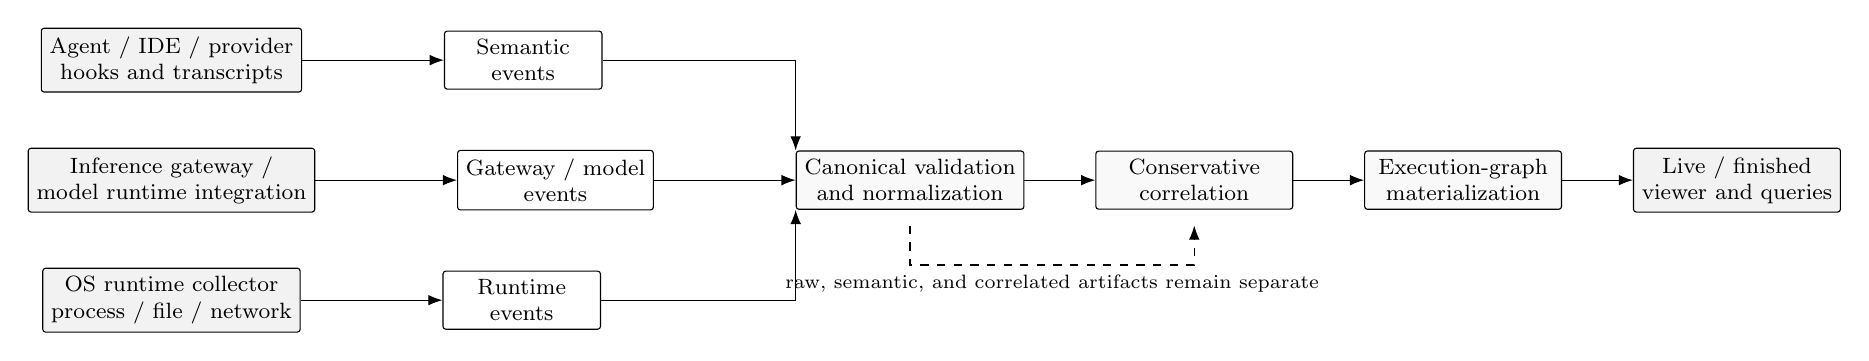
\begin{tikzpicture}[
  node distance=7mm and 9mm,
  b/.style={draw, rounded corners=1pt, align=center, minimum height=7mm, minimum width=20mm, inner sep=3pt, font=\footnotesize},
  e/.style={-{Latex[length=1.8mm]}, thin},
  d/.style={-{Latex[length=1.8mm]}, dashed, thin}
]
\node[b, fill=gray!10] (provider) {Agent / IDE / provider\\hooks and transcripts};
\node[b, below=of provider, fill=gray!10] (gateway) {Inference gateway /\\model runtime integration};
\node[b, below=of gateway, fill=gray!10] (os) {OS runtime collector\\process / file / network};

\node[b, right=18mm of provider] (sem) {Semantic\\events};
\node[b, right=18mm of gateway] (mid) {Gateway / model\\events};
\node[b, right=18mm of os] (raw) {Runtime\\events};

\node[b, right=18mm of mid, minimum width=28mm, fill=gray!5] (norm) {Canonical validation\\and normalization};
\node[b, right=of norm, minimum width=25mm, fill=gray!5] (corr) {Conservative\\correlation};
\node[b, right=of corr, minimum width=25mm, fill=gray!5] (graph) {Execution-graph\\materialization};
\node[b, right=of graph, fill=gray!10] (view) {Live / finished\\viewer and queries};

\draw[e] (provider) -- (sem);
\draw[e] (gateway) -- (mid);
\draw[e] (os) -- (raw);
\draw[e] (sem.east) -| (norm.north west);
\draw[e] (mid) -- (norm);
\draw[e] (raw.east) -| (norm.south west);
\draw[e] (norm) -- (corr);
\draw[e] (corr) -- (graph);
\draw[e] (graph) -- (view);
\draw[d] ($(norm.south)+(0,-2mm)$) -- ++(0,-5mm) -| node[pos=0.25,below,font=\scriptsize]{raw, semantic, and correlated artifacts remain separate} ($(corr.south)+(0,-2mm)$);
\end{tikzpicture}%
}
\caption{\system architecture. Provider semantics and OS evidence enter through separate collection paths. Correlation is a derived layer rather than a rewrite of the original evidence.}
\label{fig:arch}
\end{figure*}

\subsection{Semantic collection}
Provider-level evidence can include prompts, responses, tool declarations and results, model identifiers, conversation/session identifiers, sub-agent routing, and provider-specific lifecycle events. The prototype contains specialized integrations for several coding-agent and IDE environments, including Claude Code, OpenAI Codex, Google Antigravity, Cursor, and OpenCode, as well as model-runtime and gateway integrations for local or proxied inference paths. Coverage is explicitly integration-dependent: a provider identifier such as a tool-call ID or rollout thread ID is not automatically interpreted as an OS process identity.

When an integration explicitly supplies complete content, \system can store that value in a local SHA-256 content-addressed store while placing a content reference in the event stream. ``Complete from source'' means that the value delivered by that integration point was preserved; it does not claim access to hidden model state or remote provider-side data. This distinction is necessary because agent observability often conflates completeness of the received payload with completeness of the underlying execution.

\subsection{Runtime collection}
The portable backend uses periodic process/network observation and filesystem monitoring so that the same high-level collector can run on Linux, macOS, and Windows. The portability trade-off is explicit. A process or socket whose entire lifetime falls between samples can be missed. Filesystem changes observed through portable monitoring are session-correlated and therefore non-causal with respect to a particular process unless stronger evidence exists. Absence of an event is consequently not proof that the event did not occur.

On Linux, a syscall-oriented \texttt{strace} backend provides a stronger reference path for supported executions. It can follow a traced lineage and attribute selected file and network syscalls to processes, but it is not an OS-wide monitor: activity outside the traced lineage, unsupported syscall patterns, and permission restrictions remain outside its claim. These two backends intentionally expose a fidelity/performance trade-off rather than hiding it behind one boolean ``captured'' field.

\subsection{Conservative tool-to-process correlation}
The current cross-layer correlator focuses on a common but nontrivial bridge: a semantic tool call declares a command, and runtime telemetry observes candidate processes. The algorithm first rejects command forms for which executable identity cannot be safely extracted, including shell-control constructs that can expand into multiple commands. For an eligible declaration, it searches a bounded interval for process-start or process-exec observations and compares normalized executable identity, canonical executable path when available, process command line, and argument-tail evidence.

Candidate evidence is accumulated per process. A match can be supported by execution identity, process executable metadata, command-line head, or an exact argument tail. The strongest current heuristic categories correspond to combinations of executable and command-line evidence. Importantly, candidate strength does not override ambiguity: if more than one process remains compatible, the correlation is skipped. If exactly one candidate remains, the emitted bridge records its supporting event IDs, inference method, temporal delta, and a heuristic score. It is explicitly marked \texttt{inferred=true} and \texttt{causal=false}; the score is documented as a heuristic score rather than a probability.

Figure~\ref{fig:corr} summarizes the policy.

\begin{figure}[t]
\centering
\fbox{\begin{minipage}{0.94\columnwidth}
\footnotesize
\textbf{Algorithm 1: Conservative semantic-to-process correlation}
\begin{enumerate}
  \item Parse an eligible command declaration for semantic action $s$. If shell control or executable identity is unsupported, abstain.
  \item Define a bounded observation interval using the declaration time, tool completion time when available, and a maximum window.
  \item Collect runtime process-start/exec candidates whose executable/path/command-line evidence is compatible with the declaration.
  \item Aggregate supporting event IDs and evidence predicates per process candidate.
  \item If the candidate set contains anything other than one process, return $\bot$.
  \item Emit a derived $s\rightarrow p$ bridge with method and support metadata, marking it inferred and non-causal.
\end{enumerate}
\end{minipage}}
\caption{The key policy is abstention under ambiguity. A stronger visual connection is not preferred to an unsupported claim.}
\label{fig:corr}
\end{figure}

This mechanism is deliberately narrower than arbitrary causal inference. It does not claim that temporal proximity proves execution, and it does not infer byte-level flow from the co-occurrence of file and network evidence. Stronger future backends can add stronger bridges without changing the semantics of existing weaker evidence.

\subsection{Exact identity versus causality}
Some integration points expose a shared request identity across layers. Exact identity is useful, but equality of identifiers does not necessarily prove that one event caused another. \system therefore permits a relation to record exact identity while remaining non-causal. This prevents a common provenance error in which correlation, identity, and causality are collapsed into one confidence score.

\subsection{Graph materialization and querying}
Each canonical entity ID becomes a graph node and accumulates type, display metadata, observation count, first/last times, and event types. Each source--relation--target tuple becomes an aggregated directed edge with exact occurrence count and references to supporting events. Causality is aggregated conservatively: uniformly causal support yields a causal edge; uniformly non-causal support yields a non-causal edge; and mixed support remains unknown/mixed.

The graph can be queried by node type, relation, backend, or causal status. Directed path queries operate over bounded simple paths, which is important because execution graphs may contain cycles through repeated interactions. Filtering creates a derived view rather than rewriting the source graph.

\subsection{Live and finished views}
Live execution is an incremental materialization problem. Let $E_t$ be the events incorporated by time $t$. The viewer renders a projection $P(M(E_t))$ together with presentation state such as folds, selection, and viewport transform. When execution finishes and all terminal semantic synchronization completes, the finished viewer should render $P(M(E_T))$ for the final event set $E_T$. The projection may change as nodes are folded or selected, but canonical evidence identity remains stable.

The implementation uses one graph/conversation model for live, completed, and standalone finished views. This architectural choice turns live--finished parity into a testable property rather than a best-effort screenshot comparison. It also prevents post-completion polling state from being mistaken for successful semantic synchronization.

\subsection{Semantics-aware visualization}
The execution graph is heterogeneous: a root agent, sub-agent, shared model, tool, process tree, files, and external endpoints have different semantic roles even when all are graph nodes. A single unconstrained layered layout can therefore produce high fan-in hubs, interleaved semantic groups, twisted edge bundles, and large whitespace. \system's visualization layer treats graph drawing as a constrained presentation problem informed by classical layered-layout methods~\cite{sugiyama1981hierarchical,gansner1993directed,brandes2002horizontal}. Dynamic stability is applied gently because mental-map preservation can help orientation in some tasks but is not universally beneficial~\cite{archambault2011dynamic,archambault2013mentalmap}.

The key scientific boundary is that layout optimization is downstream of evidence. It may change coordinates, edge routes, ordering, grouping, and folding; it may not create semantic or causal relations that are absent from the canonical graph. We therefore treat layout quality as a secondary human-factors dimension, not as the primary provenance contribution.


\section{Implementation}
\system is implemented as a Python 3.10+ local command-line and web-viewer system. The current repository release at the time of this draft is 0.8.22. The package can wrap an arbitrary local command for OS observation or activate provider-specific recorders when stronger semantic integration is available. A run directory can retain raw runtime events, semantic events, correlated events, materialized graphs, conversation views, content-addressed payloads, and a local integrity manifest.

\subsection{Provider-neutral event boundary}
Provider adapters are intentionally upstream of the canonical graph. Their responsibility is to translate exposed lifecycle events and content into a stable event vocabulary while preserving provider identifiers as attributes. This allows downstream graph logic to remain independent of whether the source is a hook, rollout transcript, IDE plugin, gateway event, model-runtime event, or local process collector. It also makes missing semantic coverage explicit: unsupported provider internals remain absent rather than reconstructed from the final answer.

\subsection{Failure and cleanup semantics}
Observability software changes the system it observes and must therefore define failure ownership. The portable collector distinguishes terminal states such as available, degraded, unavailable, not sampled, and not requested for network collection. If a managed collector fails after launching a workload it owns, cleanup is responsible for terminating that owned workload instead of leaving an accidental child behind. Conversely, a descendant that legitimately outlives the root command is not assigned a fabricated exit event merely to close the graph. These distinctions are relevant to both runtime correctness and evaluation under interruption.

\subsection{Privacy and integrity boundary}
Local-first storage reduces default disclosure but does not make captured data harmless. Full-fidelity provider payloads can contain prompts, source code, secrets, tool outputs, file contents, and model responses. The content store is therefore part of the sensitive run artifact. A local integrity manifest can detect changes relative to a recorded manifest, but if both evidence and manifest remain in the same writable trust boundary, this is not an adversary-resistant trusted logging mechanism. The system is an observability tool, not a sandbox or trusted execution environment.

\section{Evaluation Methodology}
A journal evaluation must establish more than feature coverage. We separate \emph{descriptive comparison}, which asks what each system documents and exposes, from \emph{controlled comparative experiments}, which run equivalent workloads and measure the resulting evidence. Table~\ref{tab:rqs} defines seven research questions.

\begin{table*}[t]
\centering
\caption{Research questions and primary metrics for the controlled evaluation.}
\label{tab:rqs}
\footnotesize
\begin{tabular}{p{0.7cm} p{4.8cm} p{8.8cm}}
\toprule
RQ & Question & Primary measurements \\
\midrule
RQ1 & How faithfully does \system reconstruct execution structure? & Typed node/edge precision and recall, semantic coverage, runtime-evidence recall, graph edit distance to ground truth. \\
RQ2 & How accurately does cross-layer attribution connect semantic actions to runtime effects? & Attribution precision/recall/F1, abstention rate, ambiguity rate, and false-attribution rate under concurrency. \\
RQ3 & What evidence does \system add over representative agent-observability systems? & Common-workload coverage for agent/tool/model/process/file/network entities and ability to answer causal-attribution tasks. \\
RQ4 & Is the canonical graph stable across providers and operating systems for logically equivalent workloads? & Typed graph agreement, relation agreement, unmatched-node/edge rate, provider/OS interaction effects. \\
RQ5 & What runtime, memory, storage, and visualization overhead does observation impose? & Wall-clock overhead, peak RSS delta, artifact bytes, event throughput, live-update latency, rendering latency versus graph size. \\
RQ6 & How robust is reconstruction under adverse execution conditions? & Fidelity under short-lived processes/sockets, interrupts, exceptions, surviving descendants, missing hooks, shared resources, and degraded collectors. \\
RQ7 & Does cross-layer visualization improve human debugging and accountability tasks? & Task accuracy, time-to-root-cause, inspected events, confidence calibration, and subjective workload/usability. \\
\bottomrule
\end{tabular}
\end{table*}

\subsection{Baselines}
We propose two baseline families.

\textbf{Product/system baselines.} The competitive set should include at least Langfuse, Phoenix, W\&B Weave, and one of LangSmith or AgentOps, using the latest publicly documented instrumentation paths at experiment freeze time. AgentGraph and AgentSeer should be included where their artifacts can ingest the same traces without semantic distortion. The purpose is not to force every product to solve the same problem; it is to quantify which questions can be answered from each resulting trace representation.

\textbf{Scientific ablations.} To isolate the value of cross-layer reconstruction, the most important baselines are: (B0) semantic instrumentation only; (B1) OS-runtime observation only; (B2) naive fusion by temporal window and process ancestry without the conservative uniqueness/evidence policy; and (B3) full \system. B2 is essential because the paper's hypothesis is not merely that ``more telemetry is better.'' It is that evidence-aware fusion reduces unsupported attribution compared with a plausible but naive join.

\subsection{Fair competitor instrumentation tiers}
A direct product comparison can be misleading if one system is evaluated with extensive custom instrumentation while another is evaluated only with its default integration. We therefore separate three instrumentation tiers and report them independently.

\textbf{Tier 0---native/default.} Each product is configured using its documented agent or framework integration and its standard local or hosted collector, without adding experiment-specific OS spans. This tier measures what an ordinary user obtains from the system's intended observability path.

\textbf{Tier 1---documented extensibility.} We permit official manual-instrumentation and OpenTelemetry interfaces when they are part of the product documentation. The experiment may add spans around the deterministic workload, but the added span must be produced at an application boundary that the system documents. This tier tests whether a platform's extensible trace model can answer additional questions without an independent machine observer.

\textbf{Tier 2---common external evidence.} Where technically possible, the same independently generated OS observations are exported to a competitor as custom spans or events. This is not a comparison of native collection; it is an isolation test for representation, query, and attribution logic. If a platform can store an externally supplied process/file/network event but still requires the experimenter to decide which agent span owns it, that distinction is reported explicitly. Conversely, if a competitor provides a documented mechanism that performs the association itself, it is credited as cross-layer attribution.

These tiers prevent two symmetrical errors. Evaluating only Tier~0 can understate the expressive power of a general telemetry platform. Evaluating only Tier~2 can overstate native observability by supplying the competitor with precisely the cross-layer evidence that the experiment is intended to measure. Product cost, account tier, sampling policy, retention, and exporter configuration are frozen in the artifact manifest because they may influence the available trace.

\subsection{Diagnostic question benchmark}
Beyond node and edge counts, each reconstructed run is evaluated by a fixed set of questions whose answers are derived from an independent workload manifest. This makes the comparison task-oriented: a system receives credit only when its recorded evidence supports the answer, not merely because its UI contains visually similar entities. Table~\ref{tab:questions} defines the initial question set.

\begin{table*}[t]
\centering
\caption{Diagnostic questions used to compare semantic tracing, OS tracing, naive fusion, competitor systems, and \system. Each answer is scored against an independently generated workload manifest.}
\label{tab:questions}
\footnotesize
\setlength{\tabcolsep}{4.5pt}
\begin{tabular}{p{0.75cm} p{4.5cm} p{4.4cm} p{5.2cm}}
\toprule
ID & Diagnostic question & Required evidence & Principal failure being exposed \\
\midrule
Q1 & Which agent or sub-agent invoked a given tool action? & Semantic agent/tool identity and parentage & Missing or flattened agent hierarchy \\
Q2 & Which OS process realized a declared tool execution? & Semantic declaration plus independently observed process identity & Unsupported timestamp/process-name association \\
Q3 & Which logical action is supported as the source of a file mutation? & File evidence, process evidence where causal, and justified cross-layer bridge & Treating session-correlated filesystem activity as process-causal \\
Q4 & Which logical action is supported as the source of a network connection? & Endpoint/socket evidence, process identity, and justified cross-layer bridge & Attributing a shared or concurrent network effect to the wrong agent \\
Q5 & Which runtime effects cannot be uniquely attributed? & Candidate/support metadata and an explicit unknown/abstention state & Hiding ambiguity by forcing graph connectivity \\
Q6 & Does the finalized run preserve the evidence visible at live completion? & Canonical event and graph identities from both materializations & UI/viewer divergence mistaken for provenance consistency \\
\bottomrule
\end{tabular}
\end{table*}

For Q2--Q5, an answer is categorized as \emph{correct}, \emph{incorrect}, \emph{explicitly unknown}, or \emph{not represented}. This four-way outcome is more informative than binary answerability. ``Explicitly unknown'' indicates that a system represented the relevant evidence but declined an unsupported association; ``not represented'' indicates that the necessary entity or relation was absent. For accountability tasks these outcomes have different consequences and should not be collapsed.

\subsection{Ablations and negative controls}
The evaluation includes controlled ablations that target the mechanism of the paper rather than generic software components. The \emph{semantic-only} ablation removes independent OS evidence; the \emph{runtime-only} ablation removes provider semantics. A \emph{timestamp-only} fusion associates every semantic action with the closest compatible runtime event within the same window. A \emph{no-abstention} variant chooses the highest-scoring process even when several candidates remain. An \emph{exact-ID-only} variant disables heuristic correlation and therefore measures how much coverage can be obtained without inferred bridges. Additional feature ablations remove canonical executable paths, command-line-head evidence, and argument-tail evidence from the correlator.

These ablations separate three possible explanations for good results. If semantic-only tracing answers the cross-layer questions, independent OS evidence is unnecessary for that workload. If timestamp-only fusion performs as well as \system under concurrency, the conservative attribution mechanism adds little. If disabling abstention increases recall without increasing false attribution, the uniqueness rule is too conservative. The expected contribution is therefore a \emph{precision--coverage frontier}, not a claim that one configuration dominates on every metric.

Negative controls are equally important. We include unrelated background processes with similar executable names, a semantically declared command that intentionally never executes, shell constructs rejected by the parser, and concurrent commands with intentionally indistinguishable observable features. In these cases the correct output may be no edge. A method that maximizes graph density will fail these controls even if it appears strong on positive-only workloads.

Sampling is evaluated as an explicit treatment variable for the portable backend. Observation intervals are swept across a predeclared range while workload lifetimes are controlled independently. The resulting detection curve quantifies where short-lived process and network events become unreliable. The syscall-oriented Linux backend serves as a stronger lineage-scoped reference condition, not as universal OS ground truth.

\subsection{Primary hypotheses and statistical analysis}
The empirical study tests four primary hypotheses. \textbf{H1} states that combining semantic and independent runtime evidence increases correct answerability of cross-layer diagnostic questions relative to either evidence plane alone. \textbf{H2} states that conservative attribution reduces false-attribution rate relative to naive temporal fusion under concurrent and ambiguous execution, with an explicit trade-off in abstention or recall. \textbf{H3} states that, for logically equivalent workloads and evidence classes available on each platform, the canonical semantic relation structure is substantially more stable across providers and operating systems than raw integration-specific telemetry. \textbf{H4} states that observation cost depends strongly on backend fidelity and workload duration; fixed-cost microbenchmarks and realistic sessions should therefore be reported separately.

For proportion metrics such as attribution precision, recall, false attribution, and diagnostic-answer accuracy, the study reports point estimates with confidence intervals and the underlying counts rather than percentages alone. Paired or clustered bootstrap intervals are used when repeated runs share a workload fixture. Runtime and memory distributions are summarized with medians and tail quantiles in addition to means; paired differences are preferred when an observed and unobserved run use the same deterministic fixture. Provider and OS effects are analyzed with workload as a blocking factor rather than pooling all events into one pseudo-independent sample.

For the human study, participant and task are modeled as repeated factors. Binary correctness can be analyzed with a mixed-effects logistic model, while completion time can use a log-transformed mixed-effects model or a robust nonparametric paired analysis if model assumptions fail. The analysis plan, exclusion rules, and primary endpoints should be fixed before examining the final study results. Secondary visualization measures---for example edge-crossing count or layout compactness---remain secondary unless they predict analyst task performance.

The study should also report effect sizes that have an operational interpretation. For attribution, a reduction in false edges per run is easier to interpret than a significance test alone. For debugging, median seconds saved per correctly solved task and the change in confidence calibration are more informative than a standalone usability score. Statistical significance is therefore treated as support for a practically meaningful effect, not as the definition of usefulness.

\subsection{Version freezing and reproducibility of comparisons}
Every comparison row is bound to a versioned experiment manifest containing the system version or commit, integration package versions, account/service tier when relevant, exporter configuration, sampling policy, OS build, Python/runtime versions, model endpoint, and workload revision. Documentation-based capability tables are frozen on a stated access date, while empirical claims are tied to the exact executable configuration used in the experiment. If a competitor changes materially during the study, the primary table remains on the frozen version and a sensitivity rerun may be reported separately.

This discipline is especially important in the agent-observability ecosystem, where product interfaces and instrumentation conventions change quickly. It also prevents a subtle reproducibility failure in which a future rerun silently uses a more capable competitor release or a different provider integration and is then compared against old numbers.

\subsection{Ground-truth workloads}
The evaluation should use a workload generator whose intended process/file/network effects are externally recorded, not inferred from \system output. Each scenario emits a ground-truth manifest before execution and uses deterministic markers or controlled helper programs to make expected identities auditable. Workloads should include:
\begin{enumerate}
  \item single-agent single-tool execution;
  \item nested process trees with file reads and writes;
  \item local and remote network connections;
  \item root-agent to sub-agent delegation;
  \item two concurrent agents invoking the same executable;
  \item concurrent tool calls with overlapping temporal windows;
  \item shared model/runtime or shared tool resources;
  \item short-lived processes and sockets near the portable sampling boundary;
  \item exception, SIGINT/Ctrl+C, and abnormal collector termination;
  \item a descendant that outlives the observed root;
  \item semantic-hook denial or partial provider coverage; and
  \item unsupported shell constructs that should force attribution abstention.
\end{enumerate}

The concurrency cases are especially important. If Agent A and Agent B both launch the same executable at nearly the same time, a timestamp-only fusion can create a plausible but wrong edge. A correct conservative system should prefer $\bot$ until stronger identity evidence disambiguates the candidates.

\subsection{Cross-provider and cross-OS matrix}
The full matrix has four factors:
\begin{equation}
\textit{System}\times\textit{Provider}\times\textit{OS}\times\textit{Workload}.
\end{equation}
The provider set should use integrations that can be exercised reproducibly on the evaluation hosts; candidate families include supported coding agents and local model paths. The OS set is Windows, Linux, and macOS for the portable collector, with Linux additionally evaluated using the stronger syscall-oriented backend. Equivalent workload manifests, not identical UI screenshots, define the cross-platform unit of comparison.

For two canonical graphs $G_i$ and $G_j$ generated from the same logical workload, we report typed node agreement and typed relation agreement after matching platform-specific runtime identities through the ground-truth manifest. Raw PIDs and filesystem syntax are therefore not expected to match literally. What should match is the logical relation pattern that the platform can support at the same evidence grade.

\subsection{Attribution metrics}
Let $A^*$ be the set of ground-truth semantic-to-runtime relations and $\hat A$ be the emitted attributed relations. We report
\begin{align}
P_A &= \frac{|\hat A\cap A^*|}{|\hat A|},\\
R_A &= \frac{|\hat A\cap A^*|}{|A^*|},\\
FAR &= \frac{|\hat A\setminus A^*|}{|\hat A|}.
\end{align}
$FAR$ is the false-attribution rate. Because abstention is intentional, we also report
\begin{equation}
AR=\frac{|\{s:\phi(s)=\bot\}|}{|S_{eligible}|}.
\end{equation}
A system that never attributes anything can trivially obtain zero false attribution, so precision must be interpreted jointly with recall and abstention. Conversely, a system that connects every temporally nearby process may obtain high recall while producing unacceptable false attribution under concurrency.

\subsection{Graph fidelity}
Node and edge metrics are reported by type. This avoids a large number of easy process nodes masking poor recall for rarer but semantically important sub-agent or network relations. We additionally report a normalized typed graph-edit distance against the manifest-derived ground-truth graph and analyze errors by evidence channel.

For runtime evidence, negative claims are scoped to the backend. A portable sampling miss is counted against recall for the experiment but is not interpreted as proof that the event did not occur. The Linux syscall backend provides a useful stronger-reference condition for quantifying portable blind windows.

\subsection{Performance and scalability}
Performance experiments use paired runs of the same deterministic workload with observation disabled and enabled. Primary measures are wall-clock time, peak process-tree resident memory, artifact size, and event throughput. Viewer experiments separately vary graph nodes, edges, high-degree shared resources, and update frequency, measuring materialization time, layout time, DOM size, interaction latency, and dropped/late updates. This separation prevents an expensive graph layout from being incorrectly attributed to the collector and prevents collector overhead from being hidden by a long model call.

\subsection{Robustness experiments}
Robustness evaluation is fault-oriented rather than anecdotal. We inject or deterministically model: a short-lived child between portable process samples; a short-lived socket between network samples; a surviving/reparented child; portable filesystem activity without process-causal support; hook unavailability; malformed or incomplete semantic input; root interruption; collector failure after child launch; and ambiguous command/process matches. For each case, the expected outcome includes not only what should be observed but what \emph{must not} be claimed.

\subsection{Human-subject study}
RQ7 compares at least two interfaces: a conventional agent trace/log view and the \system cross-layer graph with evidence details. Participants perform controlled tasks such as identifying which agent caused an unexpected file change, determining which sub-agent contacted an endpoint, locating the process responsible for a tool failure, and distinguishing direct from inferred evidence. We measure correctness, completion time, number of inspected records, and confidence calibration. A within-subject counterbalanced design reduces between-participant variability. Because dynamic-graph literature shows task-dependent effects of layout stability~\cite{archambault2011dynamic,archambault2013mentalmap}, visualization claims should be tied to concrete navigation and attribution tasks rather than subjective aesthetics alone.


\section{Repository-Backed Preliminary Characterization}
This section intentionally reports only measurements for which a frozen repository artifact exists. It is not presented as the final performance evaluation of the current implementation.

\subsection{Reference microbenchmark}
The repository contains a v0.6.0 reference microbenchmark captured on GitHub Actions using a 4-logical-CPU Intel Xeon Platinum 8573C environment with 15.99~GB memory and Python~3.12.14. The deterministic workload performs file read/write/hash operations and short-lived Python subprocesses. Seven iterations were recorded per profile. Table~\ref{tab:prelim} reproduces the values statically from that artifact.

\begin{table}[t]
\centering
\caption{Repository reference microbenchmark from ExecWeave v0.6.0 (seven iterations). These are historical preliminary measurements, not claimed performance of v0.8.22.}
\label{tab:prelim}
\footnotesize
\setlength{\tabcolsep}{3.5pt}
\begin{tabular}{lrrrr}
\toprule
Profile & Median ms & Overhead & $\Delta$RSS MB & Artifact KB \\
\midrule
Off & 236.221 & 0.000\% & 0.000 & 0.000 \\
Portable & 391.580 & 65.768\% & 27.852 & 741.355 \\
Strace & 1226.076 & 419.038\% & 37.653 & 572.838 \\
\bottomrule
\end{tabular}
\end{table}

These numbers should not be generalized to long-running agent sessions. The workload is intentionally short, so fixed startup and instrumentation costs dominate the percentage. They are nonetheless scientifically useful for two reasons. First, they show that observation is not free and that the stronger syscall-oriented backend can impose substantially larger costs on this workload. Second, they prevent a future paper from reporting only favorable long-duration workloads. The final evaluation should rerun the benchmark on the submission artifact, add realistic multi-minute agent workloads, and report both absolute and relative overhead.

\subsection{Executable fidelity contracts}
The repository also encodes several observability limits as deterministic regression tests rather than documentation alone. The threat-model contract covers short-lived processes, short-lived sockets, surviving descendants, non-causal portable filesystem events, and a corresponding stronger syscall-trace case. This is methodologically important: limitations are part of the executable specification. The final paper should report the complete frozen test matrix and continuous-integration environments, but it should not substitute unit-test pass counts for empirical fidelity experiments against independent ground truth.

\subsection{What remains before a submission-quality evaluation}
Three result sets are intentionally absent from this first manuscript. First, contemporary competitor tools have not yet been run under one frozen workload harness, so Table~\ref{tab:systems} is positioning based on published interfaces rather than a performance ranking. Second, the current 0.8.22 implementation requires a fresh cross-OS/provider quantitative campaign rather than reusing acceptance-test summaries collected during development. Third, human debugging utility has not yet been measured in a controlled study. These are the highest-priority empirical tasks for a submission-ready revision.

\section{Discussion}
\subsection{The graph is a claim surface, not merely a view}
An execution graph is persuasive because edges visually imply relationships. That makes graph construction a claim boundary. If a system draws a tool directly to a process, users naturally interpret the line as evidence that the tool caused or at least executed through that process. \system therefore treats every cross-layer edge as something that must be explainable through support metadata. This stance is stricter than treating the graph as an approximate navigation aid, but it is appropriate for debugging and security use where misattribution has operational consequences.

\subsection{Why abstention is a feature}
Machine-learning interfaces often reward completeness, whereas provenance requires epistemic discipline. Equation~\ref{eq:phi} makes $\bot$ a normal output. An unattributed process is less visually satisfying than a connected graph, but it communicates a real limitation: the available evidence cannot distinguish candidates. Future instrumentation can resolve the ambiguity without invalidating the earlier record. By contrast, a fabricated edge can contaminate downstream root-cause analysis and analyst trust.

\subsection{Compatibility with OpenTelemetry}
The proposed model is not an argument against OpenTelemetry. OpenTelemetry is a natural transport and semantic source for instrumented agent and service operations~\cite{otel2026}. The key design question is whether the evidence was emitted by the application, independently observed at runtime, or derived by correlation. A future interoperability layer could ingest OTel spans as $C_{sem}$ or $C_{gw}$ events while preserving independent $C_{os}$ observations. Cross-layer links could then use propagated trace/span context as strong identity support when available and fall back to conservative runtime evidence otherwise.

\subsection{Cross-platform fidelity is necessarily asymmetric}
A portable collector cannot truthfully promise kernel-equivalent fidelity across Windows, macOS, and Linux using only common user-space APIs. \system therefore favors a common canonical schema with backend-specific evidence strength over pretending that all platforms expose identical telemetry. The scientific comparison should ask whether the graph correctly represents what each backend can support, not whether every backend emits the same number of edges.

\subsection{Remote execution boundaries}
Local OS observation stops at the local machine. A call to a remote hosted model can expose local client/network evidence and provider-supplied semantic content, but it cannot reveal the provider's remote process tree unless the provider supplies additional telemetry. Similarly, an OpenRouter or gateway identity can link logical request stages without making the remote service process locally observable. These boundaries must remain explicit in any accountability claim.

\subsection{Security analysis versus maliciousness inference}
The execution graph can support rule-based analysis---for example, identifying a process that accesses an unexpected path and later opens a network connection. Such a pattern is a finding supported by evidence; it is not proof of exfiltration or malicious intent. File and network co-occurrence does not establish byte-level flow. Evidence grade and behavioral severity should therefore remain orthogonal.


\section{Threats to Validity}
\subsection{Construct validity}
``Attribution correctness'' depends on the ground-truth definition. A semantic tool can indirectly cause a process through wrappers or schedulers, making immediate parentage different from causal responsibility. The evaluation must therefore define relation types precisely---e.g., direct execution, delegated execution, shared-resource use---rather than reduce every relation to one binary edge. Ground-truth manifests should be independently generated and audited.

Feature comparisons have another construct threat: a general tracing platform can often represent custom process/file/network spans even if it does not collect them natively. We therefore use ``not native'' rather than ``unsupported'' when official documentation lacks an independent OS collector, and controlled experiments should distinguish default instrumentation from deliberately extended custom instrumentation.

\subsection{Internal validity}
Provider integrations evolve quickly. A result measured with one release may reflect an integration bug rather than a conceptual limitation. All comparative experiments must freeze versions, configuration, model endpoints, and workload seeds/fixtures. For nondeterministic model-driven workloads, the OS side effects should be induced by deterministic tool scripts after the agent chooses a known action, or the study should replay a fixed semantic trace into the execution harness.

Timing-sensitive runtime tests can also be flaky. Blind-window experiments should model observation schedules deterministically where possible and complement real-time stress tests rather than rely only on ``sleep for $n$ milliseconds'' assumptions.

\subsection{External validity}
The supported coding-agent and local-runtime integrations do not represent every agent architecture. Browser agents, mobile agents, Kubernetes-hosted agents, serverless tool execution, and remote sandboxes introduce different visibility boundaries. The proposed evidence model should generalize, but the implementation and measurements may not. Similarly, developer workstations differ from production clusters in workload scale and privilege constraints.

\subsection{Conclusion validity}
Performance distributions can be heavy-tailed, especially when model/network latency dominates. Relative overhead should therefore be measured on deterministic local workloads as well as realistic agent sessions, report medians and tail statistics, and include sufficient repetitions. Human-study claims require power analysis and appropriate mixed-effects or repeated-measures statistics rather than relying on a small convenience sample.

\section{Reproducibility, Ethics, and Data Handling}
The public implementation should be accompanied by a frozen artifact containing workload generators, environment manifests, competitor configuration instructions that comply with each system's license and service terms, raw metric outputs, and scripts that compute reported statistics. The manuscript itself should contain static final numbers and must not depend on executing external data-loading code during typesetting.

Observability studies can capture sensitive prompts, source code, authentication material, file contents, and network destinations. Experimental workloads should therefore use synthetic repositories and controlled endpoints whenever possible. Human-subject evaluation should avoid collecting participants' real agent histories. Any released trace corpus should be generated for the study or reviewed for secrets before publication.

A further ethical issue is attribution. A graph that names an agent or process can be interpreted as assigning responsibility. The interface should preserve evidence grade, inference status, and ambiguity so that derived correlation is not presented as forensic certainty. This is both a systems-design requirement and a reporting requirement for the research artifact.

\section{Future Research Directions}
The present design opens several research questions beyond the initial system paper. First, propagated cryptographic or trace identities could reduce ambiguity without relying on command matching, but require adoption across agent, tool, gateway, and model-runtime boundaries. Second, learned correlation could potentially improve recall, yet any learned model would need calibrated abstention and auditable evidence features to avoid replacing a transparent heuristic with opaque false attribution. Third, whole-system provenance backends such as LSM/eBPF-style collectors could strengthen Linux evidence while retaining the canonical cross-layer model. Fourth, distributed agents require provenance across machines and trust domains, bringing the problem closer to X-Trace and distributed provenance but with agent identities as first-class principals. Finally, graph-layout evaluation could become a separate human-factors study focused on shared-resource hubs, semantic group continuity, and dynamic orientation rather than generic crossing counts.

\section{Conclusion}
Agent observability is rapidly becoming graph-based, but a graph of application spans is not the same object as a graph that connects semantic agent actions to independently observed machine effects. \system treats this distinction as the central problem. It preserves provider semantics, gateway/model evidence, and OS runtime telemetry as separate evidence channels; materializes them into one typed execution graph; and makes cross-layer attribution conservative, inspectable, and explicitly fallible. The design prefers an unattributed effect to a convenient but unsupported edge and separates evidence strength from behavioral severity.

This formulation positions \system between two mature traditions: application/distributed tracing, which excels at instrumented logical workflows, and whole-system provenance, which excels at machine-level dependency histories. Agentic software increasingly needs both. A submission-quality evaluation must therefore measure not only how many nodes a dashboard can display, but whether the system reconstructs the right entities and relations, abstains when evidence is ambiguous, remains consistent across providers and operating systems, survives adverse execution conditions, imposes acceptable cost, and materially improves human debugging and accountability tasks. The first manuscript establishes that model and the controlled evaluation protocol; the next empirical revision should fill those questions with frozen, reproducible measurements rather than product-feature inference.


\balance
\bibliographystyle{IEEEtran}
\bibliography{references}

\end{document}
